\documentclass[../main.tex]{subfiles}

\begin{document}

\section{Alcantarilla}

\subsection{Determinación del Caudal}

Debido a la ventaja de no requerir datos hidrométricos para la determinación de caudales máximos de una cuenca se utilizó  el "Método Racional Generalizado". Los datos del proyecto son:

\begin{figure}[h]
    \centering
    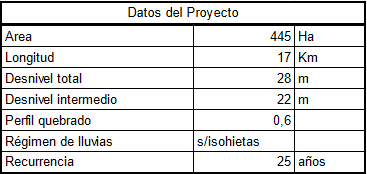
\includegraphics{images/google_sheets/Screenshot_6.png}
    \caption{Datos del proyecto}
    \label{fig:datos_proyecto}
\end{figure}

Además, sabemos que:
\begin{equation*}
    \text{Caracteristicas} \longrightarrow
        \begin{cases} 
            \text{Monte poco tupido, poco permeable - Loam Arcilloso $85\%$ - Loam $15\%$} \\
            \text{Cauce poco sinuoso, sección aproximadamente uniforme,} \\ \text{arbustos y algo de malezas.}
        \end{cases}
\end{equation*}

\begin{equation*}
    \text{Rugosidad}  \longrightarrow \text{Corriente concentrada en cauces naturales.}
\end{equation*}

\addtocontents{toc}{\protect\setcounter{tocdepth}{1}}
\subsubsection{Longitud de la cuenca}
\addtocontents{toc}{\protect\setcounter{tocdepth}{3}}

Se determinó la distancia entre el punto más alejado de la cuenca y el de desagüe, medido a lo largo del cauce principal , en kilómetros 

\addtocontents{toc}{\protect\setcounter{tocdepth}{1}}
\subsubsection{Rugosidad de la Cuenca}
\addtocontents{toc}{\protect\setcounter{tocdepth}{3}}

Para obtener la rugosidad de la cuenca se utilizó el Cuadro 1


\addtocontents{toc}{\protect\setcounter{tocdepth}{1}}
\subsubsection{Desnivel y Tiempo de Concentración}
\addtocontents{toc}{\protect\setcounter{tocdepth}{3}}


Según el método adoptado, el desnivel presentado por la cuenca corresponde al caso C: Cauce con perfil quebrado ($\eta > 0,70$), y para su determinación se nos propone en \cref{desnivel}, la cual, sumada al método de semejanza de triángulos nos brindará el nivel correspondiente.

\begin{equation}
     H=2*\eta *Hc + (1-\eta)* Hr \label{desnivel}
\end{equation}

Luego, con los datos obtenidos se ingresó en el gráfico Nº 5 y se adoptó el tiempo de concentración correspondiente.

\addtocontents{toc}{\protect\setcounter{tocdepth}{1}}
\subsubsection{Precipitación Horaria}
\addtocontents{toc}{\protect\setcounter{tocdepth}{3}}

Se determinó la Precipitación Horaria en milímetros/ horas según la figura Nº6 "Mapa de curvas isohietas de la República Argentina" 

\addtocontents{toc}{\protect\setcounter{tocdepth}{1}}
\subsubsection{Intervalo de Recurrencia}
\addtocontents{toc}{\protect\setcounter{tocdepth}{3}}

Es el período de tiempo que en promedio transcurre para que la magnitud de un fenómeno hidrológico sea igualada o sea superada una vez en dicho período, en nuestro caso es un dato ya brindado.

\addtocontents{toc}{\protect\setcounter{tocdepth}{1}}
\subsubsection{Intensidad de la lluvia}
\addtocontents{toc}{\protect\setcounter{tocdepth}{3}}

Se la determinó como la media puntal correspondiente al intervalo de recurrencia adoptado

\subsubsection{Cuadro resumen}

De todos los cálculos anteriores, podemos desarrollar el siguiente cuadro resumen presentado en \cref{fig:cuadro_resumen}, con los valores obtenidos. Para lo mismo se utilizó el Método Racional Generalizado. \cite{metodo_racional}

\begin{figure}[ht]
    \centering
    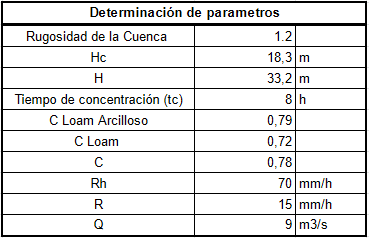
\includegraphics[width=0.5\textwidth]{images/google_sheets/Screenshot_7.png}
    \caption{Cuadro resumen}
    \label{fig:cuadro_resumen}
\end{figure}

\subsection{Dimensionamiento}

Se dimensionará una alcantarilla de hormigón tipo cajón con alas a 45º. Para ello se obtuvieron los coeficientes de rugosidad de Manning (gráfico Nº 6) y de pérdida de carga a la entrada (gráfico Nº 20) $\eta$ y $K_e$ respectivamente.\cite{alcantarilla} 

\begin{figure}[h]
    \centering
    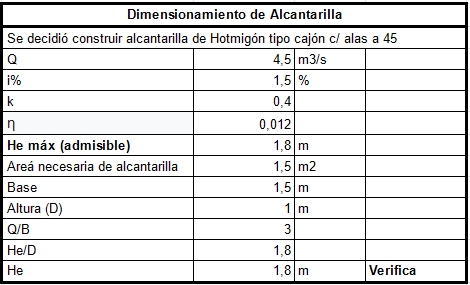
\includegraphics[width=0.5\textwidth]{images/google_sheets/Screenshot_18.png}
    \caption{Dimensionamiento}
    \label{fig:Dimensionamiento1}
\end{figure}

\begin{figure}[h]
    \centering
    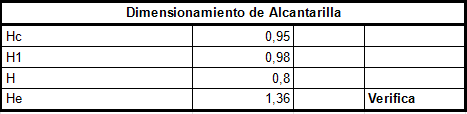
\includegraphics[width=0.5\textwidth]{images/google_sheets/Screenshot_19.png}
    \caption{Dimensionamiento}
    \label{fig:Dimensionamiento2}
\end{figure}

\addtocontents{toc}{\protect\setcounter{tocdepth}{1}}
\subsubsection{Control de Entrada}
\addtocontents{toc}{\protect\setcounter{tocdepth}{3}}
 Se estimó una sección transversal inicial como el cociente entre el caudal dado y la velocidad máxima. Luego se ingresó en el gráfico Nº1 (He/D) con el fin de una verificación, como la alcantarilla no cumplía lo requerido, se aumentaron las dimensiones de la misma y se volvió a verificar. De esta forma, mediante un proceso iterativo se adoptó un valor de altura de entrada máximo admisible.
 
\addtocontents{toc}{\protect\setcounter{tocdepth}{1}}
\subsubsection{Control de Salida}
\addtocontents{toc}{\protect\setcounter{tocdepth}{3}}

Para la verificación del control de salida se utilizaron las siguientes expresiones:

\begin{align}
H_e &= H + H_1 - L_{xi} \\
H_1 &= \frac{(h_c + D)}{2}
\end{align}

Para determinar $H_1$, primero se calculó la altura crítica ($h_c$), la cual se la obtuvo del gráfico 15. Luego, del gráfico 8, se determinó la altura de carga ($H$). 
Finalmente se compararon las entradas He(salida) y He(entrada) y se determinó que la alcantarilla trabajará con un control de entrada 

\addtocontents{toc}{\protect\setcounter{tocdepth}{1}}
\subsubsection{Verificación}
\addtocontents{toc}{\protect\setcounter{tocdepth}{3}}

Finalmente se realizó la verificación de velocidad a la salida del conducto utilizando la fórmula de continuidad.

\begin{figure}[h]
    \centering
    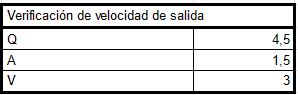
\includegraphics[width=0.4\textwidth]{images/google_sheets/Screenshot_20.png}
    \caption{Verificación}
    \label{fig:verificacion}
\end{figure}

\addtocontents{toc}{\protect\setcounter{tocdepth}{1}}
\subsubsection{Alcantarilla Adoptada}
\addtocontents{toc}{\protect\setcounter{tocdepth}{3}}


\begin{figure}[h]
    \centering
    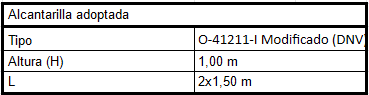
\includegraphics[width=0.5\textwidth]{images/google_sheets/Screenshot_21.png}
    \caption{Alcantarilla adoptada}
    \label{fig:alcantarilla_adoptada}
\end{figure}

\addtocontents{toc}{\protect\setcounter{tocdepth}{1}}
\subsubsection{Longitud Necesaria del Conducto}
\addtocontents{toc}{\protect\setcounter{tocdepth}{3}}

Dada las cotas laterales y del eje del camino, existe una longitud del conducto que no posee quiebres, ubicada justo debajo de la tapada mínima.
Para el cálculo de la longitud necesaria de conducto se utilizaron las siguientes expresiones: 

\begin{equation}
J = A_C + 0.50+3*[T - (0.40 * F)]
\end{equation}

La flecha la obtenemos desde la siguiente ecuación:

\begin{equation}
F = [A*i(\%)] + [A_{\text{b}}*i_{\text{b}}(\%)]  
\end{equation}

Donde: \\
$J$: Longitud necesaria\\
$A_C$: Ancho de coronamiento. \\
$A$: Ancho carril. \\
$A_b$: Ancho banquina.\\
$i$: Pendiente del carril. \\
$i_b$: Pendiente de la banquina.\\
$T$: Tapada.\\
$F$: Flecha \\


Obteniendo una longitud de conducto de: 

\begin{equation}
    J =  (3.65+3.5)*2 + 0.5 + 3*(2.01-0.4*0.213)
\end{equation}
\begin{equation}
    J =  20.6 \text{m}
\end{equation}


\end{document}